\documentclass[12pt]{article}
\title{Smart Agriculture: Water Management}
\author{Chandler Scott}
\date{\today}

\usepackage{graphicx}
\usepackage{geometry}
\usepackage{subcaption}
\geometry{
  left=3cm,
  right=3cm,
  top=2cm,
  bottom=2cm
}
\begin{document}

\maketitle
\clearpage
%%%%%%%%%%%%%%%%%%%%%%%%%%
\section{Introduction}\label{sec:intro}
This report presents the development and simulation of a wireless sensor network for smart agriculture water management, specifically designed to optimize irrigation in crop fields. As global water resources come under increasing pressure, the need for efficient agricultural practices becomes more critical. This project utilizes the OMNet++ network simulator alongside the INET framework to model a system of soil moisture sensors and irrigation actuators that respond dynamically to changes in soil moisture levels. By automating irrigation based on precise, real-time data, the system aims to reduce water waste, enhance crop yield, and promote sustainable agricultural practices. This introduction outlines the simulated setup, the methodology for data collection and analysis, and the potential for future advancements in smart agriculture technology.

%%%%%%%%%%%%%%%%%%%%%%%%%%
\section{Scenario Description}\label{sec:scenario}
This scenario envisages a crop field equipped with a state-of-the-art wireless sensor network aimed at optimizing irrigation practices. The network consists of eight sensor nodes distributed strategically across the field. Each node is equipped with a soil moisture sensor and an irrigation actuator.

The primary goal of this setup is to ensure efficient water usage by automatically adjusting irrigation based on the real-time soil moisture levels detected by the sensors. This system facilitates precise water management, where irrigation is dynamically adapted to the needs of specific areas within the field, preventing both overwatering and under-watering.

When the server detects that a sensor's soil moisture level in its vicinity has fallen below a critical threshold—indicative of the need for water—it messages the corresponding sensor's irrigation actuator to trigger water that specific area. This targeted irrigation approach not only conserves water but also promotes optimal crop health and growth by maintaining ideal soil moisture conditions throughout the growing season.

The centralized control system, which manages the sensor inputs and actuator outputs, ensures that each section of the crop field receives attention as needed, based on the real-time data provided by the sensors. This intelligent management system represents a significant advancement over traditional irrigation methods, which often rely on preset schedules and uniform application of water across large areas, regardless of specific ground conditions.

In summary, this scenario showcases a technology-driven approach to agriculture that leverages advanced sensor technology and automated systems to enhance irrigation efficiency and sustainability in crop production.

%%%%%%%%%%%%%%%%%%%%%%%%%%
\begin{figure}[ht!]
  \centering
  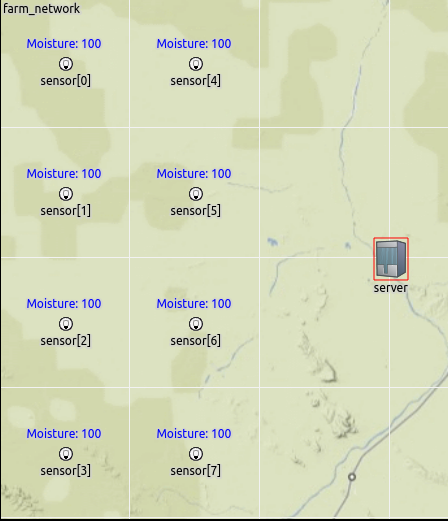
\includegraphics[width=0.8\linewidth]{images/smart_farm.png}  
  \caption{Smart Farm Simulation Setup}
  \label{fig:sim} 
\end{figure}
\section{Simulation Setup}\label{sec:sim}
To simulate smart agriculture water management, the network simulator OMNet++ along with the INET framework was employed. The simulation setup includes eight wireless devices equipped with soil moisture sensors and irrigation actuators, and a central server that controls the irrigation based on soil moisture data over a 24 hour period. The soil moisture update frequency and dissemination interval to the server are configurable; the default settings update soil moisture every twenty seconds and disseminate readings every ten minutes. Initially, soil moisture is set at one hundred percent, with a minimum threshold of zero. If the moisture level falls below fifty percent, the server commands the device to activate its irrigation system. These parameters—update frequency, dissemination interval, and moisture threshold—are adjustable through OMNet++.

The network communication is managed using UDP for data transmission and CSMA/CD for access control, with the option to configure acknowledgements (ACKs) in the simulation settings. This flexibility allows for testing the robustness and efficiency of the system under various network reliability scenarios.

\begin{figure}[ht!]
  \centering
  \begin{subfigure}[b]{0.45\textwidth}  % The "b" aligns subfigures at the bottom
    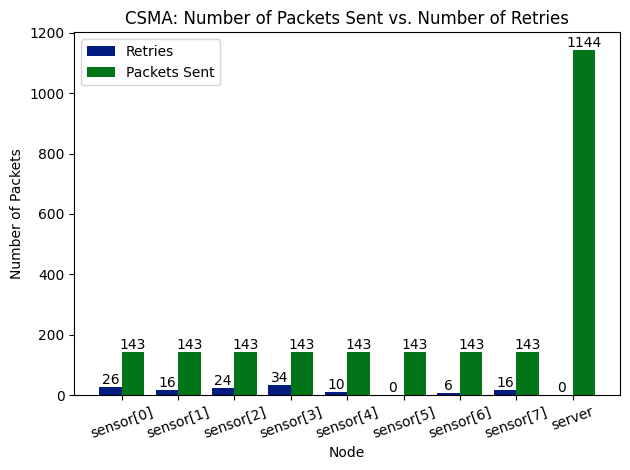
\includegraphics[width=\textwidth]{images/ack.png}
    \caption{CSMA with ACK}
    \label{fig:ack}
  \end{subfigure}
  \hfill  % Adds horizontal space between the figures
  \begin{subfigure}[b]{0.45\textwidth}
    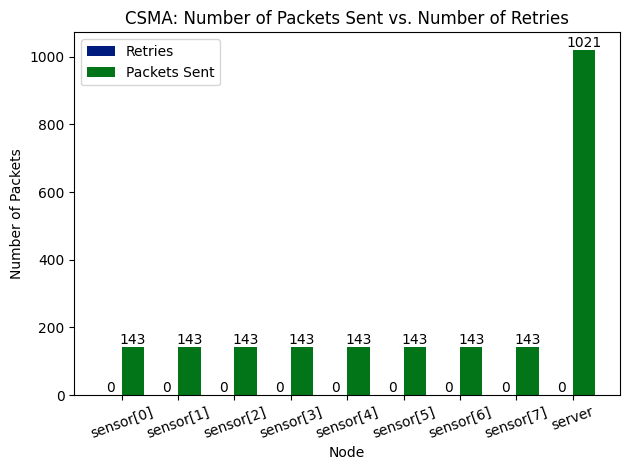
\includegraphics[width=\textwidth]{images/noack.png}
    \caption{CSMA with No ACK}
    \label{fig:noack}
  \end{subfigure}
  \caption{Simulation Metrics}
  \label{fig:analysis}
\end{figure}
%%%%%%%%%%%%%%%%%%%%%%%%%%
\section{Data Analysis}\label{sec:data}
For data analysis, the focus was on evaluating the packet delivery rates and the number of retry attempts in the CSMA-based communication between sensors and the server, both with and without acknowledgements (ACKs). When ACKs were enabled, the packet delivery ratio achieved a perfect 100\%. In contrast, disabling ACKs resulted in a lower packet delivery ratio of 89.24\%. This discrepancy highlights the critical role of ACKs in ensuring reliable data transmission in wireless sensor networks.

The analysis also quantified the communication overhead introduced by ACKs. Enabling ACKs led to an additional 110 messages being retransmitted (from 1144 total messages) to confirm packet receipt. This increased communication not only affects the network's traffic load but also significantly impacts the energy consumption of the sensor devices. The higher energy expenditure associated with ACKs and retransmissions is a key consideration, especially in energy-constrained environments typical of wireless sensor networks.

Understanding these trade-offs is crucial for optimizing network protocols in terms of reliability and energy efficiency. Future optimizations might explore adaptive ACK strategies, where the use of acknowledgements could be dynamically adjusted based on network conditions or the criticality of the data being transmitted, thereby balancing reliability with energy usage.


%%%%%%%%%%%%%%%%%%%%%%%%%%
\section{Future Work}\label{sec:future}
Future studies could enhance the central server's decision-making process by integrating artificial intelligence (AI). Currently, the system activates irrigation based on a predefined soil moisture threshold. By employing AI, this threshold could be dynamically adjusted to maintain optimal soil conditions, tailored to specific crop needs. Additionally, AI could incorporate external data, such as weather forecasts, to predict future soil moisture levels more accurately. This would allow the irrigation system to preemptively adjust to changing environmental conditions, optimizing water usage and enhancing crop management.

%%%%%%%%%%%%%%%%%%%%%%%%%%
\section{Conclusion}\label{sec:conclusion}
In conclusion, the simulation of a wireless sensor network for irrigation management has demonstrated significant potential to improve water usage efficiency in agriculture. The system's ability to respond to real-time soil conditions ensures that water is distributed more precisely, which is crucial for conservation efforts and for meeting the agricultural demands of an increasing global population. The findings from packet delivery and communication retries have provided valuable insights into the trade-offs between system reliability and energy efficiency, which are essential considerations in the deployment of wireless sensor networks in resource-constrained environments. Looking forward, the integration of artificial intelligence could further refine the system's responsiveness and predictive capabilities, ultimately leading to even more robust agricultural management systems. This research not only advances our understanding of smart irrigation technologies but also contributes to the broader field of sustainable agriculture.

\end{document}
